
\documentclass[12pt,fleqn,leqno,letterpaper]{article}
\usepackage[utf8]{inputenc}
\usepackage[english]{babel}

\usepackage{hyperref}
\usepackage{graphicx}
\usepackage{minted}

\usepackage{tikz}
\usetikzlibrary{shapes.geometric,positioning}

\include{preamble}


\title{Assignment 2}
\author{Anders L. Hurum\\
    \small{Development of Real-Time Systems}\\
    \small{EIT Digital}\\
    \small{\texttt{andershurum@gmail.com}}
}
\date{\today}

\begin{document}


    \maketitle

    \begin{abstract}

        The second assignment for the Real-Time systems course consisted of developing
        an application for exploring how priorities, executiontime, periods influence eachother
        in practise in a Real-Time system. \\ \\
        For more details on the assignment, see the \texttt{assignment\_2.md} document
        in the repository at github. \\

        \url{http://github.com/peakbreaker/tuts\_FreeRTOS}

    \end{abstract}

    \newpage

    \section*{Introduction}
        To fullfill the requirements by the assignment it is planned to implement the RTOS
        with three tasks:

        \begin{itemize}
            \item prioritysettask
            \item matrixtask
            \item communicationtask
        \end{itemize}

        The idea is that matrixtask will be responsible charge of matrix calculations, while
        communicationstask will handle communication to a peripheral (like transmitting the calculations from matrixtask).
        Finally prioritysettask will measure and manage the tasks, and set priorities according to the requirements
        of our application. \\

        \begin{figure}[h]
            \centering
            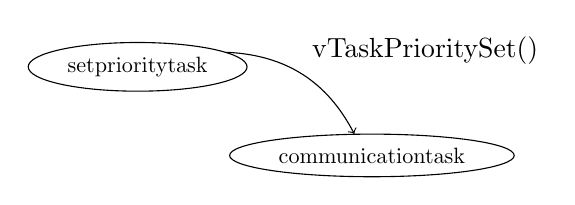
\begin{tikzpicture}
                    \node (l1) [ellipse, draw=black, fill=white!20, text=black, scale=0.8]{
                    setprioritytask};
                    \node (l3) [ellipse, draw=black, fill=white!20, text=black, scale=0.8, below right=1cm of l1]{
                    communicationtask};
                \draw[bend left,->]  (l1) to node [auto] {vTaskPrioritySet()} (l3);
            \end{tikzpicture}
            \caption{Tasks}
            \label{figure:tasks}
        \end{figure}

        We aim with this to answer questions relating to execution priorities in FreeRTOS,
        and find out how priorities, periods and pre-emptiveness influence the behavior of
        execution in Real Time systems.

    \section*{Code}

        Worth noting in the code is that the task handlers are avaliable to all tasks in the main program file.
        Also important is the variables for time and task activation.  These variables are incremented by the
        tick interrupt routine when the tasks are active. The reason for this is to provide us with the ability
        to inspect the amount of time that the tasks have been active, so we can implement the prioritysettask correctly.
        Thus we implement the main program like this, note here the handlers and timer variables.

        \begin{minted}{c}
/* Handlers for the tasks */
TaskHandle_t matrix_handle = NULL;
TaskHandle_t communication_handle = NULL;
TaskHandle_t priority_handle = NULL;

/* Timers for the tasks */
long matrix_ticks = 0;
long comm_ticks = 0;
boolean matrix_active = FALSE;
boolean comm_active = FALSE;

/*-----------------------------------------------------------*/

int main(void)
{
    prvInitialiseHeap();

    vTraceInitTraceData();
    xTickTraceUserEvent = xTraceOpenLabel("tick");

    /* Create the tasks */
    xTaskCreate((pdTASK_CODE)matrix_task, (signed char *)"Matrix", 1000,
        NULL, 3, &matrix_handle);
    xTaskCreate((pdTASK_CODE)communication_task, (signed char *)"Communication",
        configMINIMAL_STACK_SIZE, NULL, 4, &communication_handle);
    xTaskCreate((pdTASK_CODE)prioritysettask, (signed char *)"Priority",
        configMINIMAL_STACK_SIZE, NULL, 5, &priority_handle);

    // This starts the real-time scheduler
    vTaskStartScheduler();

    // Should not reach here
    for ( ;; );

}
        \end{minted}

        Since we were given the matrixcalculation task and communicationtask, we will simply
        look here at how we implemented the prioritysettask:

        \begin{minted}{c}
static void prioritysettask()
{
    static int comm_pri = 4;    // Using a local variable -> less api calls
    static int comm_time = 0;	// Variable to calc ticks -> time in ms
    printf("Priority set task has been initialized...\n");
    fflush(stdout);
    while (1) {
        // First calculate the communications time in ms
        comm_time = comm_ticks * portTICK_PERIOD_MS;
        // Uncomment for debug purposes
        //printf("PriSetTask getting COMTIME    : %i ms...\n", comm_time);
        //fflush(stdout);
        /* LOGIC : In the execution of this task we check the active ticks
            * for the communication task - if over 1000 ms, we raise priority,
            * while under 200 ms, we lower priority */
        if (comm_time > 1000 && comm_pri != 4) {
            comm_pri = 4;
            printf("Communication task running slowly at %i ms,
                    increasing priority to 4\n", comm_time);
            fflush(stdout);
            vTaskPrioritySet(communication_handle, comm_pri);
        }
        else if (comm_time < 200 && comm_pri != 2) {
            comm_pri = 2;
            printf("Communication task running fast enough at %i ms,
                    reducing priority to 2\n", comm_time);
            fflush(stdout);
            vTaskPrioritySet(communication_handle, comm_pri);
        }
        // -- Block the task for some ticks before we loop --
        vTaskDelay(1000);
    }
}
        \end{minted}

        Since the prioritysettask should only run after we have gotten the exectutiontime of communicationtask,
        the communication task will suspend the prioritysettask when running, and reset the ticks variable. \\

    \section*{Results}

        The resulting output from the program were as follows : \\

        \begin{figure}[h]
            \centering
            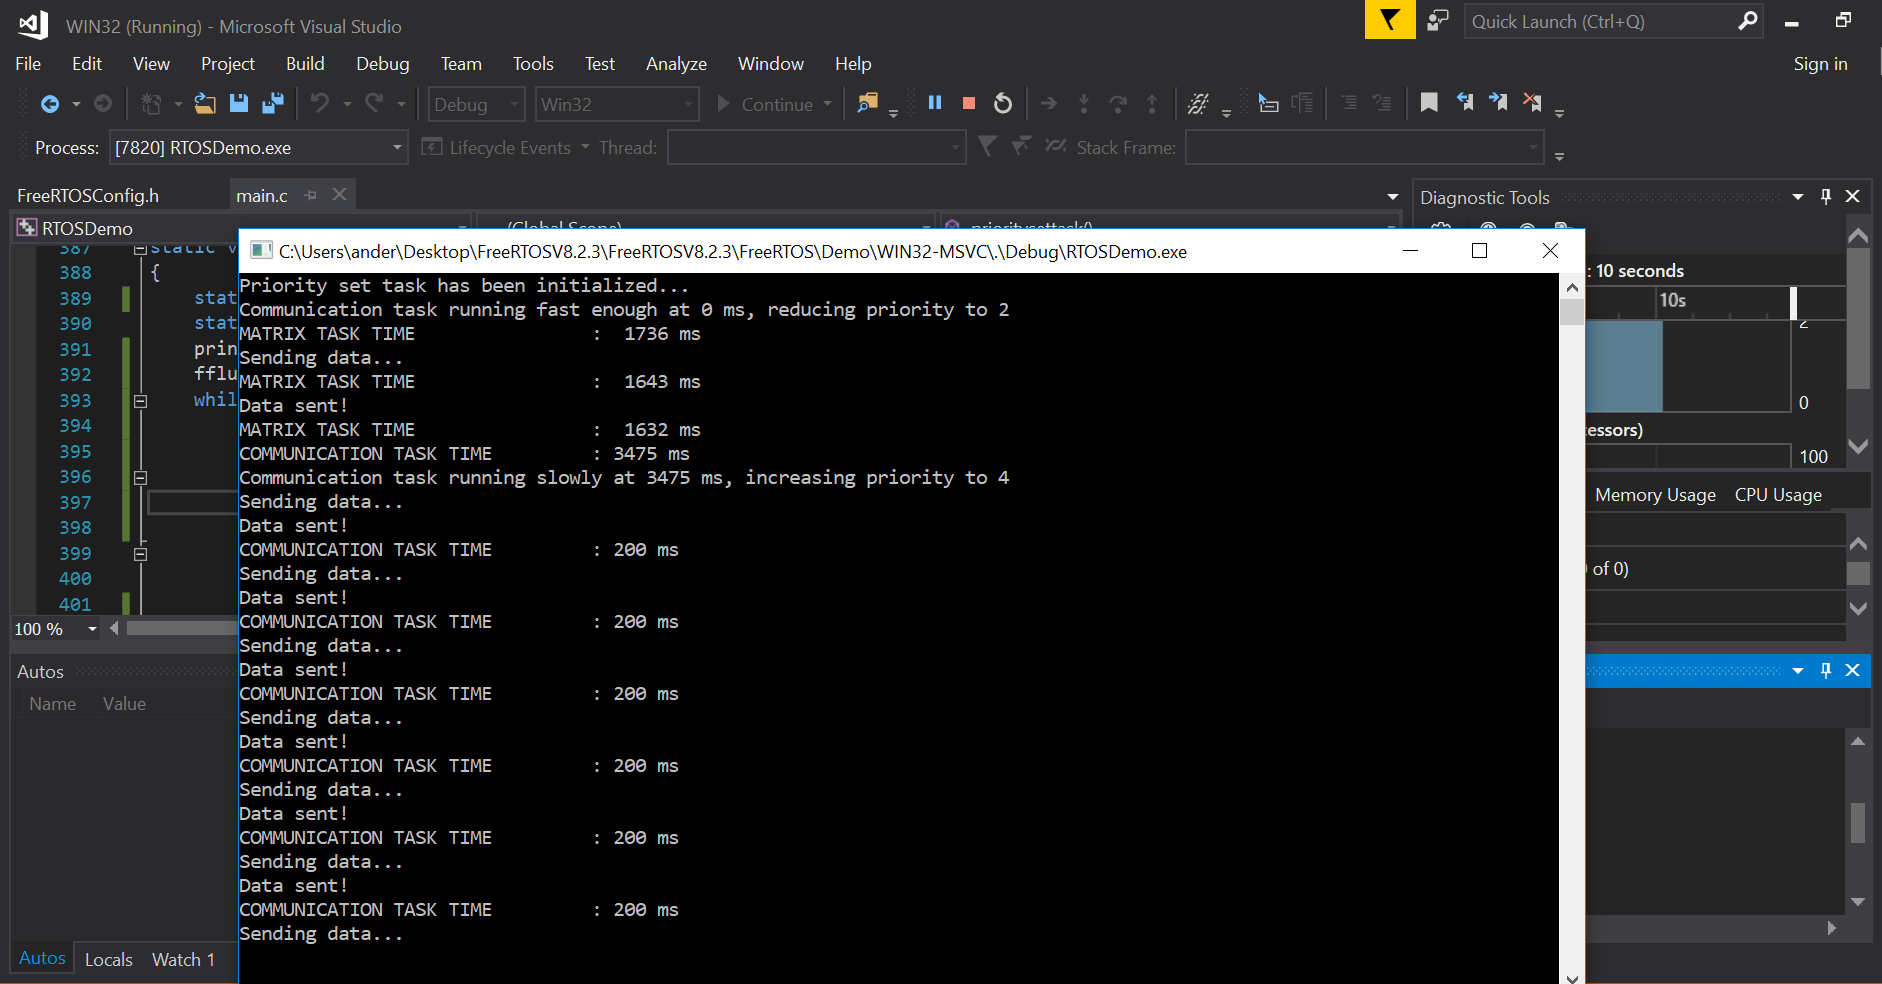
\includegraphics[width=\textwidth]{Debug_1.png}
            \caption{Debug output}
            \label{figure:debug1}
        \end{figure}

        As seen in the debug output, when the program initializes the exec time of communicationstask is set to 0,
        so its priority is quickly set to 2.  This causes the matrixcalculation task to block the communication task, which causes
        its time to be over 3000 ms.  Therefore after its execution, its priority is increased, which causes it to
        consecutively execute at a little over 200 ms. \\

        More interestingly though is in the case when I change the code of prioritysettask to change the prirotiy of
        the communication task if its executiontime is less than 220 ms rather than 200 ms.  This causes its priority
        to be changed every other time it executes.  This was not the requirement, just an interesting experiment with
        real time systems.  The following is the output from this scenario:

        \begin{figure}[h]
            \centering
            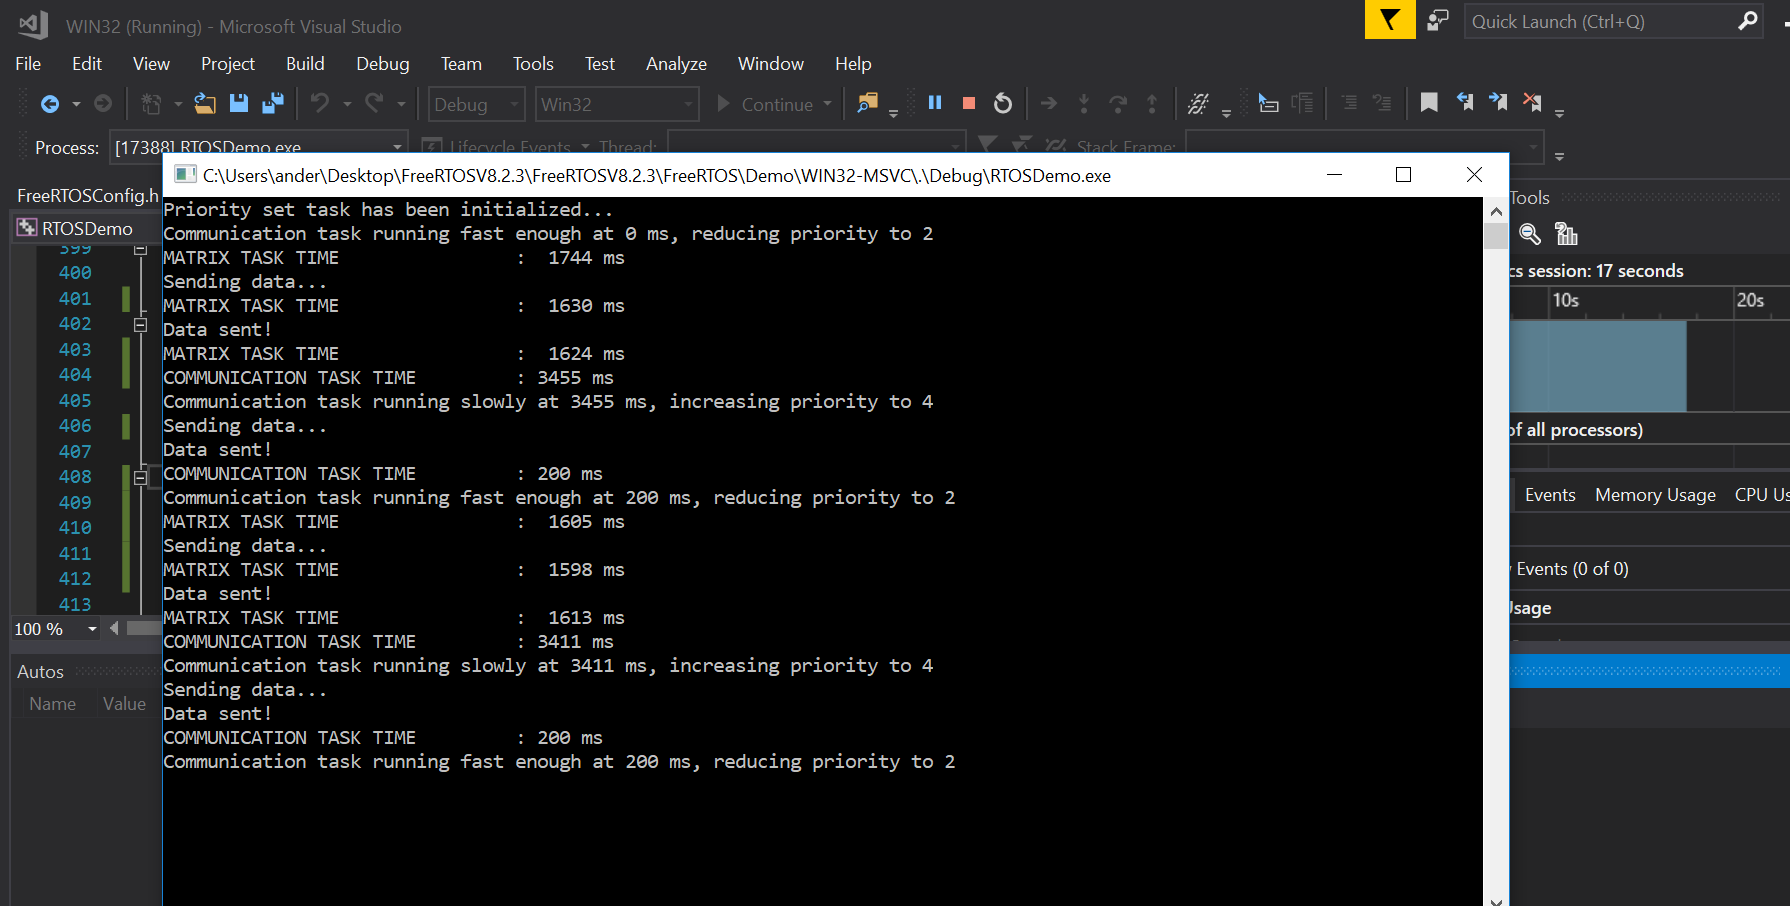
\includegraphics[width=\textwidth]{Debug_2.png}
            \caption{Debug output}
            \label{figure:debug2}
        \end{figure}

    \section*{Learning outcome}
        \begin{itemize}
            \item \textbf{Why is "matrixtask" using most of the CPU utilization?}

        The matrix task is more computationally expensive than the other tasks, and its priority is higher.

            \item \textbf{Why must the priority of "communicationtask" increase in order for it to work properly}

        The matrix task is blocking the communicationtask from executing due to it having a higher priority, and that it is
        computatuinally expensive, so it takes a while to execute. Therefore, for communicationtask to run properly, its must
        increase priority, so it can pre-empt the matrixtask.

            \item \textbf{What happens to the completion time of "matrixtask" when the priority of "communicationtask" is increased?}

        There seems to be very little difference, which is expected as commuincationtask consumes very little computational resources

            \item \textbf{How many seconds is the period of "matrixtask"? (Hint: look at vApplicationTickHook() to measure it)}

        Currently the code is measuring executiontime.  To measure period, I removed the use of the matrix\_active boolean, and just reset the
        matrix\_ticks variable every time the matrixtask ran.  The code at the beginning of the matrix task thus looks like this:

        \begin{minted}{c}
printf("MATRIX TASK TIME  :  %i ms \n", matrix_ticks * portTICK_PERIOD_MS);
fflush(stdout);
matrix_ticks = 0;
        \end{minted}

        After this we get a period at about 1.7 sec.

        \end{itemize}

    \end{document}
